Включим все измерительные устройства и компьютер.
Устанавливая сцинтилляционный счётчик под разными углами $\theta$ к первоначальному
направлению полёта $\gamma$-квантов, снимем амплитудные спектры с помощью ЭВМ.
На экране ЭВМ отметим пиковые значения спектра и занесём полученные результаты в таблицу.

\begin{table}[h!]
  \centering
  \caption{Результаты измерений фотопиков.}
  \import{./}{meas_table.tex}
\end{table}

Обработаем экспериментальные данные и занесём в таблицу.
По ним построим график зависимости (\ref{img::chart})
$1 - \cos{\theta}$ от $\frac{1}{N(\theta)} \cdot 10^3$, данная зависимость,
согласно теоретической \eqref{1b} будет линейной.

\begin{table}[h!]
  \centering
  \caption{Обработанные экспериментальные данные.}
  \label{exp}
  \import{./}{exp.tex}
\end{table}

\begin{figure}[h!]
  \centering
  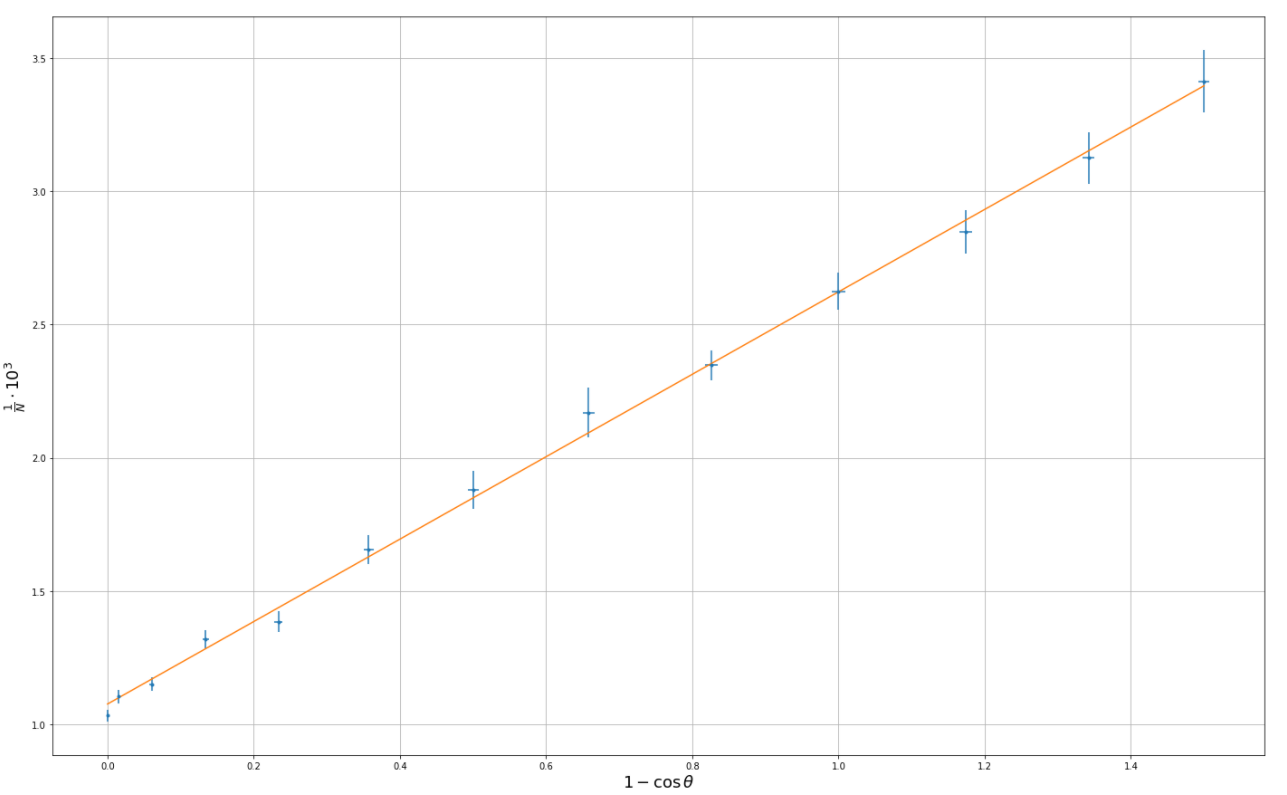
\includegraphics[width=0.9\linewidth]{one_div_n.png}
  \caption{График зависимости $1 - \cos{\theta}$ от $\frac{1}{N(\theta)}\cdot 10^3$.}
  \label{img::chart}
\end{figure}

Методом наименьших квадратов получим значение для коэффициента наклона
$A = 1.55 \pm 0.02$, а также для коэффициента $b = 1.076 \pm 0.015$ в
зависимости вида
$$
\frac{10^3}{N(\theta)} = A \cdot \left(1 - \cos{\theta}\right) + b
$$
Используя формулу \eqref{2}, а также полученную зависимость,
получим значение для энергии покоя частиц, на которых происходит
комптоновское рассеяние
$$
\boxed{
mc^2 = 460 \pm 14 \: \text{кэВ}
}
$$
